\documentclass[11pt]{article}
\usepackage[utf8]{inputenc}
\usepackage{amsmath}
\usepackage{graphicx}
\usepackage[section]{placeins}
\usepackage{float}
\graphicspath{ {/} }
%Gummi|065|=)
\title{\textbf{Universidad Nacional de Costa Rica \newline \newline Facultad de Ciencias Exactas y Naturales \newline \newline Escuela de Informática \newline \newline Paradigmas de Programación \newline \newline Proyecto 1}}



\author{\newline Grupo 1 \\\\ Omar Segura Villegas \\ Carlos Artavia Pineda \\ Fabián Hernández Chavarría \\ Andrey Campos Sánchez}
\date{}
\renewcommand*\contentsname{Contenidos}
\renewcommand{\figurename}{Figura}
\begin{document}

\maketitle

\begin{figure}[h] 

\includegraphics[scale=0.5]{logouna}
\centering
\end{figure}
\begin{flushright}
Documento Resumen del Proyecto \\ Heredia, 2016
\end{flushright}

\newpage

\tableofcontents

\newpage

\section{Introducción}
El siguiente es el reporte del primer proyecto del curso Paradigmas de Programación, donde se desarrolló una aplicación tipo cliente-servidor utilizando el modelo SPA (single page application), y también utilizando diferentes herramientas y tecnologías como Node.js y Express.js para el servidor junto con la base de datos MongoDB.\\
	Cabe resaltar que, se utilizó el patrón de diseño MVC (modelo, vista, controlador) tanto en el servidor como en el cliente donde se refleja una sólida estructura de proyecto, todo esto enfocado en los principios de programación funcional.\\

\newpage

\section{Problema planteado}
\begin{itemize}
	\item Generar en el cliente o servidor, a solicitud del usuario, un laberinto automáticamente de distinta complejidad usando algoritmos eficientes.
	\item Resolver un laberinto generado de manera manual o automática a solicitud del usuario mostrando en forma apropiada la solución.
	\item Salvar (persistir) el estado de la aplicación local o remotamente para uso futuro según el usuario lo demande.
\end{itemize}
	
\section{Resolución}
La manera de resolución fue la planteada en clase por el profesor, una aplicación web de tipo cliente-servidor, donde en el cliente se utilizó el estándar de paginas web HTML con el modelo-vista-controlador. En la vista se muestran una serie de botones, añadidos con bootstrap, framework de CSS, que responden a una serie de eventos que envían peticiones de forma asíncrona al servidor, lo cual hace que la página sea concurrente y no se bloquee el hilo de ejecución principal del navegador. \\
	Para el manejo de eventos, se utilizó jQuery, una biblioteca de Javascript para simplificar la manera de interactuar con los elementos del DOM.\\
	Al enviar las peticiones al servidor, se aplican promesas de ES6 para evitar el \textit{código spaguetti} con los callbacks y para visualizar mejor el flujo de trabajo de los algoritmos.\\
	Con respecto al servidor se empleó express como framework de Node.js para la infraestructura del servidor, y por último se implementó la persistencia de datos en MongoDB. A continuación un esquema que ilustra lo anteriormente mencionado.\\

\begin{figure}[H] 
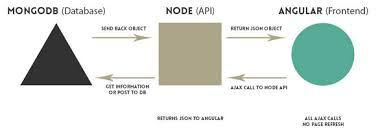
\includegraphics[scale=1.0]{mongo}
\centering
\caption{clase Maze.js}
\end{figure}

\section{Algoritmos importantes}
La generación del laberinto se resolvió por medio del algoritmo de backtracking como idea principal, donde se tiene una clase “Maze” que a su vez  contiene un grid que es un conjunto de objetos celda que se construyen a partir del nivel que el usuario seleccionó, por medio de tamaños predeterminados previamente. \\
	El algoritmo va  generando celdas en posición aleatoria hasta que se cumpla con el tamaño del grid, hay que tomar en cuenta que cada celda tiene “paredes” que son los cuatro lados de la celda y por medio de estas se define si se dibujan o no con algoritmos de ayuda como la función “quitar paredes”, que elimina las paredes necesarias para que tome forma de laberinto.\\


\begin{figure}[H] 
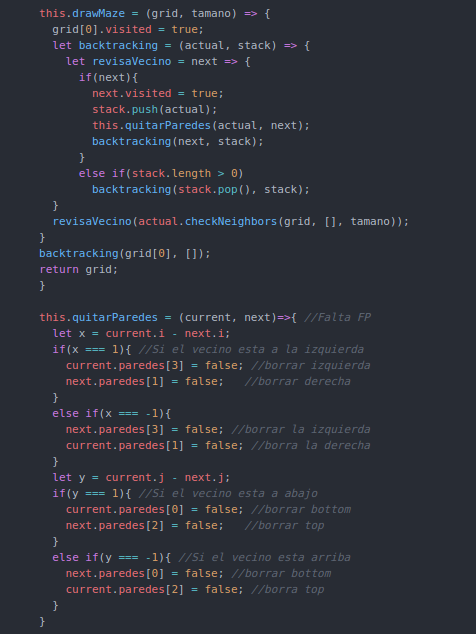
\includegraphics[scale=0.5]{maze}
\centering
\caption{clase Maze.js}
\end{figure}

\begin{figure}[H] 
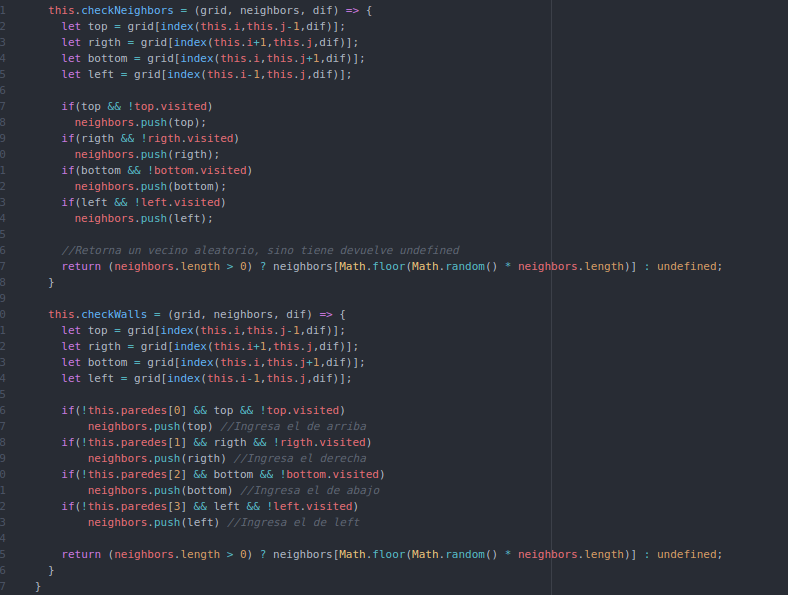
\includegraphics[scale=0.5]{cell}
\centering
\caption{clase Cell.js}
\end{figure}

Ahora bien, lo anterior es la parte lógica ya que para la generación gráfica se utiliza otro algoritmo que por medio de canvas pintan el laberinto en la página, este lo que hace es revisar para cada celda si “existen” la paredes y las dibuja. \\

\begin{figure}[H] 
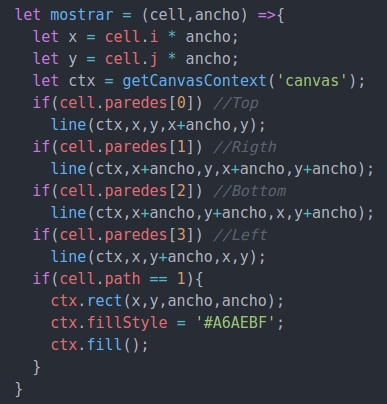
\includegraphics[scale=0.5]{draw}
\centering
\caption{Método de muestra hacia el canvas}
\end{figure}

La solución automática utiliza el mismo algoritmo de backtracking y va guardando en una variable path si la celda fue visitada, hasta que esté en la última posición del grid. Luego para dibujarlo se verifica si cada celda del grid tiene la variable path en 1 o verdadera y se pinta con el método mostrar que está anteriormente, a continuación el algoritmo de resolver el laberinto automáticamente.

\begin{figure}[H] 
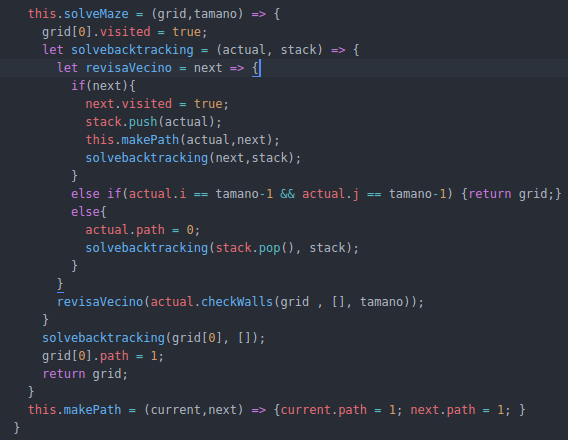
\includegraphics[scale=0.5]{solve}
\centering
\caption{Método de solución del laberinto}
\end{figure}


Por último para la solución manual del laberinto se utilizó un método que responde a los eventos generados por las flechas, y este pinta la celda en la que se encuentra, para ello, se utiliza una clase cursor para saber la posicion X y Y en la que se encuentra el jugador.


\section{Conclusiones}
La mayor comodidad que sintió el grupo de trabajo fue por poder trabajar con Javascript tanto en el servidor como en el cliente, ya que no hay que hacer conversiones de tipos de objetos como pasaba en tecnologías como servlets de Java. \\
	También, fue muy provechoso la investigación de nuevas tecnologías como Node.js y Express.js, que están con buen auge en el mercado. Además, los fundamentos de programación funcional hacen “ponerse los lentes” y enfocarse en un paradigma al que no se estaba acostumbrado, al principio genera conflictos pero estos mismos resuelven en aprendizaje.\\


\section{Referencias}

1. NodeJs Foundation. (2016). NodeJS Docs. 11/8/2016, de Node.js Foundation. Sitio web: https://www.nodejs.org/en/ \\
2. NodeJs Foundation. (2016). Express-Node. 11/8/2016, de Node.js Foundation. Sitio web: http://www.expressjs.com/es/\\
3. MongoDB Inc.. (2016). MongoDB. 22/8/2016, de MongoDB Sitio web: https://www.mongodb.com/\\
4. Mozilla Developer Network. (2015-2016). Using Fetch. 15/8/2016, de Mozilla Developer Network Sitio web: https://www.developer.mozilla.org/\\
5. W3School. (2016). Bootstrap. 29/8/2016, de School Sitio web: http://www.w3schools.com/bootstrap/\\


\end{document}